% Manufactured Death: Mathematical Modeling of HIV Prevention Impossibility
% Among People Who Inject Drugs
% A Barrier Decomposition Analysis
% Formatted for The Lancet HIV
% Last updated: December 27, 2024

\documentclass[11pt]{article}

% Lancet HIV formatting requirements
\usepackage[margin=1in]{geometry}
\usepackage{times}
\usepackage{setspace}
\usepackage{graphicx}
\usepackage{booktabs}
\usepackage{amsmath}
\usepackage{amssymb}
\usepackage[numbers,super,sort&compress]{natbib}
\usepackage{url}
\usepackage{hyperref}
\usepackage{xcolor}
\usepackage{lineno}
\usepackage{caption}

% Lancet style settings
\doublespacing
\linenumbers
\captionsetup{labelfont=bf,font=small}

% Custom commands
\newcommand{\Rzero}{R$_0$}

\begin{document}

% TITLE PAGE
\begin{center}
{\Large\bfseries Manufactured Death: Mathematical Modeling of HIV Prevention Impossibility Among People Who Inject Drugs}

\vspace{0.5cm}

{\large\itshape A Barrier Decomposition Analysis}

\vspace{1cm}

AC Demidont, DO$^{1}$

\vspace{0.5cm}

$^1$Independent Researcher; Nyx Dynamics LLC

\vspace{0.5cm}

\textbf{Correspondence to:}\\
AC Demidont, DO\\
Nyx Dynamics LLC\\
Email: acdemidont@nyxdynamics.org

\vspace{1cm}

\textbf{Word count:} 3,500 (excluding abstract, tables, figures, references)\\
\textbf{Abstract word count:} 300\\
\textbf{Tables:} 2\\
\textbf{Figures:} 6\\
\textbf{Supplementary Figures:} 8\\
\textbf{Supplementary Materials:} S1 (Mathematical Foundations)\\
\textbf{References:} 50
\end{center}

\newpage

% ABSTRACT
\section*{Abstract}

\textbf{Background:} Long-acting injectable HIV pre-exposure prophylaxis (LAI-PrEP) achieves >99\% efficacy, yet people who inject drugs (PWID) remain excluded from FDA indications and experience near-zero prevention uptake. We developed a computational model to quantify barriers to HIV prevention among PWID and predict the timeline for stochastic avoidance failure.

\textbf{Methods:} We constructed a three-layer barrier framework decomposing HIV prevention failure into: (1) pathogen biology, (2) HIV testing limitations, and (3) architectural failures (policy, stigma, infrastructure, research exclusion, algorithmic bias). Monte Carlo simulation (n=100,000 per scenario) quantified cascade completion probability across eight policy scenarios. A stochastic avoidance failure model predicted outbreak probability incorporating methamphetamine prevalence trajectories and network density evolution. Signal-to-noise ratio (SNR) analysis quantified training data disparity for machine learning algorithms.

\textbf{Findings:} Under current policy, P(\Rzero{}=0) = 0.00\% (95\% CI: 0.00--0.00) for PWID versus 16.30\% for men who have sex with men (MSM) receiving identical pharmacological intervention---an infinite-fold disparity. Barrier decomposition attributed 93.2\% of failure to architectural barriers (policy 38.4\%, infrastructure 21.9\%, stigma 20.5\%, machine learning 8.2\%, research exclusion 4.1\%), 6.8\% to HIV testing limitations, and 0.0\% to pathogen biology. SNR analysis revealed 120-fold disparity in machine learning training data (MSM: 9,180; PWID: 76.4). The stochastic avoidance model predicted 63.3\% probability of major outbreak within 5 years (median: 4.0 years).

\textbf{Interpretation:} HIV prevention failure among PWID is structurally determined rather than pharmacologically limited. Architectural barriers create cascade attrition that drug efficacy cannot overcome. The stochastic avoidance model provides a quantitative timeline for outbreak probability, with implications for resource allocation and policy prioritization.

\textbf{Funding:} None.

\newpage

% RESEARCH IN CONTEXT
\section*{Research in Context}

\subsection*{Evidence before this study}
We searched PubMed for articles published from January 1, 2010, to December 1, 2024, using terms ``HIV prevention,'' ``people who inject drugs,'' ``PrEP,'' ``structural barriers,'' and ``HIV outbreak.'' Published evidence demonstrates PWID experience dramatically lower PrEP uptake (0--3\%) compared to MSM (>20\%) despite similar awareness. The Bangkok Tenofovir Study (2013) remains the only major PrEP trial enrolling PWID; no LAI-PrEP trial has reported results for this population. Multiple U.S. outbreaks since 2015 have occurred in settings with inadequate prevention infrastructure. Systematic reviews document criminalization, stigma, and incarceration as barriers, but no study has quantified their relative contributions or modeled outbreak probability over time.

\subsection*{Added value of this study}
This study introduces a three-layer barrier framework quantifying contributions of pathogen biology (0.0\%), HIV testing limitations (6.8\%), and architectural failures (93.2\%) to prevention failure. We demonstrate that cascade completion probability approaches zero under current policy despite 99\% drug efficacy. The signal-to-noise ratio analysis quantifies the 120-fold disparity in machine learning training data between MSM and PWID. The stochastic avoidance failure model provides the first quantitative prediction of outbreak probability over time (63\% within 5 years).

\subsection*{Implications of all the available evidence}
Architectural barriers---not drug efficacy---determine HIV prevention outcomes for PWID. The multiplicative cascade structure means no single intervention achieves meaningful improvement; comprehensive reform is required. The 63\% five-year outbreak probability quantifies the timeline for policy action. Machine learning algorithms trained on current literature will systematically deprioritize PWID due to training data imbalance.

\newpage

% INTRODUCTION
\section{Introduction}

Among the estimated 15.6 million people who inject drugs (PWID) globally, 17.8\% are living with HIV---a prevalence 22 times higher than the general population.\cite{degenhardt_global_2017} Long-acting injectable pre-exposure prophylaxis (LAI-PrEP) achieves >99\% efficacy in preventing HIV acquisition, yet PWID remain excluded from FDA indications and experience near-zero prevention uptake despite similar awareness levels to other populations.\cite{mistler_prep_2021,biello_prep_2018}

The fundamental requirement for HIV prevention is achieving a state where the basic reproductive number approaches zero (\Rzero{}$\approx$0)---sustained pharmacological protection during all potential exposure events. For PWID, achieving this state requires successful navigation of an 8-step prevention cascade: awareness, willingness, healthcare access, disclosure of injection drug use, provider willingness to prescribe, adequate HIV testing, initiation, and sustained engagement.\cite{biello_prep_2018}

We hypothesized that barriers operating at three distinct levels---pathogen biology, HIV testing algorithms, and architectural failures---create conditions where cascade completion probability approaches zero, rendering \Rzero{}=0 unachievable regardless of drug efficacy. We further hypothesized that current HIV prevention among PWID relies primarily on stochastic avoidance---probability-based prevention where transmission fails to occur due to chance rather than systematic intervention\cite{greenhalgh_stochastic_2016,bobashev_firewall_2013}---and that this mechanism is time-limited.

This analysis develops computational models to: (1) calculate cascade completion probability under current policy; (2) decompose prevention failure into constituent barrier layers; (3) compare PWID outcomes to MSM receiving identical interventions; (4) quantify signal-to-noise ratio disparity in machine learning training data; and (5) predict outbreak probability over time.

% METHODS
\section{Methods}

\subsection{Theoretical Framework}

We conceptualized HIV prevention barriers as operating at three hierarchical levels with multiplicative effects on cascade completion (see Supplement S1 for mathematical foundations):

\textbf{Layer 1 (Pathogen Biology):} HIV establishes irreversible infection within 4--72 hours of mucosal exposure and within minutes of parenteral inoculation. This layer dictates the temporal window for effective prevention.

\textbf{Layer 2 (HIV Testing Limitations):} Current testing algorithms cannot reliably detect acute infection before LAI-PrEP initiation.\cite{tanner_npep_2025} Window periods range from 10--33 days for RNA testing to 31--90 days for rapid tests. LAI-PrEP delays HIV detection by median 98 days, during which 63\% of breakthrough infections develop resistance mutations.\cite{marzinke_cabla_2023,eshleman_resistance_2022}

\textbf{Layer 3 (Architectural Failures):} Structural barriers operate through five mechanisms: (a) Policy---criminalization, with 80\% of studies showing negative effects;\cite{debeck_criminalization_2017} (b) Stigma---healthcare discrimination experienced by 78\% of PWID;\cite{muncan_stigma_2020} (c) Infrastructure---prevention systems designed for other populations;\cite{biello_prep_2018} (d) Research Exclusion---systematic exclusion from trials;\cite{brody_exclusion_2021,kamitani_bestpractices_2024} (e) Machine Learning---algorithmic deprioritization from training data imbalance.

\subsection{Cascade Model}

We modeled LAI-PrEP implementation as an 8-step cascade where sustained protection requires completion of all steps. Each step probability incorporates barrier-specific penalties:

\begin{equation}
P(\text{step}_i) = P_{\text{base},i} \times \prod_{b \in \text{barriers}} (1 - \text{penalty}_{b,i})
\end{equation}

Cascade completion probability is:

\begin{equation}
\pi_{\text{cascade}} = \prod_{i=1}^{8} P(\text{step}_i)
\end{equation}

Final P(\Rzero{}=0) incorporates incarceration survival over the analysis horizon:\cite{stone_incarceration_2018}

\begin{equation}
P(R_0=0) = \pi_{\text{cascade}} \times (1 - r_{\text{inc}})^{T}
\end{equation}

where $r_{\text{inc}}$ is annual incarceration rate (30\% for PWID) and $T$ is the time horizon (5 years).

\subsection{Monte Carlo Simulation}

We simulated 100,000 individuals per scenario over 5 years. For each individual: (1) cascade progression was determined using barrier-adjusted probabilities; (2) annual incarceration probability was applied; (3) individuals were classified as achieving \Rzero{}=0 only if completing all steps and avoiding incarceration for 5 years.

Eight policy scenarios were modeled: Current Policy, Decriminalization Only, Decriminalization + Stigma Reduction, SSP-Integrated Delivery, Full Harm Reduction, Full HR + Trial Inclusion, Full HR + ML Debiasing, and Theoretical Maximum.

\subsection{Signal-to-Noise Ratio Analysis}

For machine learning algorithms trained on HIV prevention literature, we defined signal-to-noise ratio (SNR) as (see Supplement S1 for derivation):

\begin{equation}
\text{SNR} = \frac{n \times \tau \times \pi}{\epsilon \times \mu}
\end{equation}

where $n$ = trial participants, $\tau$ = evidence tier (1.0 for direct RCT, 0.5 for extrapolated), $\pi$ = precision (inverse CI width), $\epsilon$ = extrapolation required, and $\mu$ = population mismatch factor.

\subsection{Stochastic Avoidance Failure Model}

We modeled outbreak probability as a function of network density:\cite{desjarlais_outbreak_2022}

\begin{equation}
\rho(t) = \rho_0 + m(t) \times \mu \times 0.5 + h \times 0.3 + r \times 0.2 + m(t) \times 0.15
\end{equation}

where $\rho(t)$ is network density, $m(t)$ is methamphetamine prevalence, $\mu$ is network multiplier, $h$ is housing instability, and $r$ is incarceration rate.

Methamphetamine prevalence was modeled as 14.3\% baseline (2018) with 2.5\%/year growth nationally,\cite{glick_meth_2018} with regional variation (Pacific Northwest: 35\%; Appalachia: 25\%; Northeast Urban: 12\% with 5\%/year growth). Annual outbreak probability followed an exponential function above critical threshold 0.35, with protective effects from SSP (40\% reduction) and OAT (30\% reduction) coverage.

\subsection{MSM Comparison}

MSM cascade completion was calculated using published data\cite{grant_iprex_2010} with step probabilities 75--95\% and 5\% annual incarceration rate, representing identical pharmacological intervention in a population included in trial design.

\subsection{Sensitivity Analysis}

Three analyses were conducted: (1) probabilistic sensitivity analysis (PSA) with 1,000 samples varying parameters $\pm$25\%; (2) tornado analysis identifying influential parameters; (3) barrier removal analysis quantifying incremental effects.

% RESULTS
\section{Results}

\subsection{Cascade Failure Under Current Policy}

Under current policy, the 8-step cascade showed severe attrition (Figure 1). Step probabilities were: awareness 10\%, willingness 30\%, healthcare access 35\%, disclosure 25\%, provider willing 35\%, testing adequate 45\%, first injection 45\%, sustained engagement 25\%. Product: 0.00465\%. After 5-year incarceration survival (16.8\%), P(\Rzero{}=0) = 0.000782\%.

Monte Carlo simulation (n=100,000) yielded observed P(\Rzero{}=0) = 0.00\% (95\% CI: 0.00--0.00). Of simulated individuals, 89.9\% failed at awareness.

\subsection{Barrier Decomposition}

Barrier decomposition (Figure 2) attributed: pathogen biology 0.0\%, HIV testing 6.8\%, architectural failures 93.2\%. Within architectural: policy 38.4\%, infrastructure 21.9\%, stigma 20.5\%, machine learning 8.2\%, research exclusion 4.1\%.

Pathogen biology contributed 0.0\% because cascade attrition was so severe that biological constraints were never tested.

\subsection{Signal-to-Noise Ratio}

SNR analysis (Figure 5; Supplement S1) revealed:

For MSM:
\begin{equation}
\text{SNR}_{\text{MSM}} = \frac{10,800 \times 1.0 \times 0.85}{1.0 \times 1.0} = 9,180
\end{equation}

For PWID:
\begin{equation}
\text{SNR}_{\text{PWID}} = \frac{2,413 \times 0.5 \times 0.38}{3.0 \times 2.0} = 76.4
\end{equation}

Disparity ratio: 120-fold. For LAI-PrEP specifically, PWID SNR is undefined (zero trial participants).

\subsection{Policy Scenario Analysis}

Table 1 presents results across scenarios. Decriminalization alone: 0.14\% (95\% CI: 0.12--0.17). SSP-integrated: 5.03\% (4.89--5.16). Full harm reduction: 9.42\% (9.24--9.60). Full HR + ML debiasing: 18.62\% (18.38--18.86). Theoretical maximum: 19.92\% (19.67--20.17).

\subsection{MSM vs PWID Comparison}

MSM achieved P(\Rzero{}=0) = 16.30\% versus 0.00\% for PWID (Figure 3)---infinite-fold disparity from identical pharmacological intervention. MSM cascade probabilities: 75--95\% per step. MSM incarceration survival: 77.4\%.

\subsection{Stochastic Avoidance Failure}

The model predicted 63.3\% outbreak probability within 5 years (Figure 4); median 4.0 years. By 10 years: 87.6\%. Regional variation (Table 2): Pacific Northwest 88\% (median 1.0 year); Appalachia 78\% (median 2.0 years); Northeast Urban 64\% (median 3.0 years).

\subsection{Sensitivity Analysis}

PSA confirmed robustness: mean P(\Rzero{}=0) = 0.0005\%, 90\% CI (0.00\%, 0.00\%). Tornado analysis identified baseline outbreak probability ($\pm$49.8pp), critical threshold ($\pm$17.8pp), and methamphetamine multiplier ($\pm$16.6pp) as most influential. Barrier removal: criminalization alone +0.23pp; all barriers +19.88pp.

% DISCUSSION
\section{Discussion}

\subsection{Summary of Findings}

This computational analysis demonstrates that HIV prevention failure among PWID results from architectural barriers rather than pharmacological limitations. The same LAI-PrEP intervention achieving 16.30\% sustained protection among MSM achieves 0.00\% among PWID. Barrier decomposition attributed 93.2\% of failure to architectural factors, with pathogen biology contributing 0.0\%. The stochastic avoidance model predicted 63\% outbreak probability within 5 years.

\subsection{Interpretation of Cascade Failure}

The cascade structure explains why drug efficacy is irrelevant when structural barriers prevent access. When 90\% of PWID fail at awareness, the 4--72 hour biological window for prevention is never tested. This finding aligns with expert consensus that single interventions cannot achieve epidemic control among PWID;\cite{strathdee_review_2020} the multiplicative cascade requires simultaneous intervention across barriers.

The 120-fold SNR disparity quantifies the training data imbalance for machine learning systems. Algorithms trained on HIV prevention literature receive high-precision MSM data (10,800+ participants across 9+ trials) and low-precision PWID data (2,413 participants in one oral PrEP trial; zero LAI-PrEP participants). This creates conditions for systematic algorithmic deprioritization---not through malicious design but through training set composition.

\subsection{Stochastic Avoidance and Outbreak Prediction}

The concept of stochastic avoidance provides critical context for interpreting outbreak patterns. HIV transmission requires intersection of infected source, susceptible contact, and transmission event---conditions that may fail to occur by chance.\cite{greenhalgh_stochastic_2016} Des Jarlais and colleagues demonstrated that even with 10--20\% syringe sharing, HIV can remain at low prevalence through network effects.\cite{desjarlais_hiv_2016,bobashev_firewall_2013}

Our model predicts this stochastic protection is time-limited. The 63\% five-year outbreak probability reflects network density evolution driven by methamphetamine prevalence growth and forced geographic clustering. The outbreaks in Scott County,\cite{peters_scottcounty_2016,gonsalves_scottcounty_2018} Lawrence/Lowell,\cite{alpren_massachusetts_2020} and Cabell/Kanawha Counties\cite{mcclung_cabell_2021,bonacci_kanawha_2023} occurred where stochastic protection failed. Van Handel et al. identified 220 vulnerable counties in 2016;\cite{van_handel_vulnerability_2016} only 21\% had SSPs by 2018.

\subsection{The Algorithmic Barrier and Feedback Dynamics}

The negative feedback loop depicted in Figure 6 illustrates how training data exclusion perpetuates itself. Trial exclusion produces inadequate evidence, producing algorithmic deprioritization, producing reduced access, producing poor outcomes, reinforcing the perception that PWID are ``hard to reach'' and justifying continued exclusion.

This mechanism parallels what O'Neil termed ``Weapons of Math Destruction''---algorithms that encode existing inequities into automated systems operating at scale.\cite{oneil_wmd_2016} The HIV prevention literature has inadvertently created a leave-one-out cross-validation framework at population scale: PWID are the held-out test population that was never validated.

Addressing this barrier requires intervention at the root node (trial inclusion) rather than downstream (algorithmic debiasing). Debiasing algorithms trained on exclusionary data cannot compensate for the absence of training signal. The SIMPLIFY trial (HCV) demonstrated PWID achieve equivalent outcomes (94\% vs 97\%) when included in trials;\cite{grebely_simplify_2018} the ``hard to reach'' framing is contradicted by within-company evidence.

\subsection{Structural Considerations}

The persistence of barriers despite expert warnings reflects structural factors beyond the scope of this computational analysis. Decriminalization would reduce incarceration-related cascade disruption but conflicts with criminal justice revenue streams. Prevention reduces treatment demand but conflicts with pharmaceutical revenue from lifelong antiretroviral therapy. Prior authorization creates short-term insurance savings but long-term treatment costs.

These competing interests create systemic resistance to comprehensive reform. Machine learning could theoretically assist with complex resource allocation, but only if trained on data that appropriately weights population health outcomes. Current training data produces algorithms that optimize for populations with high-quality evidence (MSM) while systematically deprioritizing populations with low-quality evidence (PWID).

\subsection{Limitations}

Cascade parameters derive from heterogeneous literature with varying methodologies; sensitivity analysis demonstrated robustness across parameter uncertainty. The stochastic model simplifies complex network dynamics; local outbreak timing depends on factors not captured in aggregate parameters. Policy scenarios represent idealized conditions; real-world implementation would involve partial and gradual changes. We assumed multiplicative barrier effects; synergistic or antagonistic interactions may exist.

\subsection{Strengths}

Strengths include: quantification of barrier contributions enabling prioritization; demonstration that identical drugs produce infinite-fold disparity based on structural factors; first mathematical prediction of outbreak probability over time; identification of algorithmic bias as emerging barrier; formal SNR analysis grounding the training data imbalance; validation through comprehensive sensitivity analysis.

\section{Conclusions}

HIV prevention among PWID is structurally determined rather than pharmacologically limited. Architectural barriers create cascade attrition that drug efficacy cannot overcome, producing 0.00\% sustained protection versus 16.30\% for MSM receiving identical intervention. The stochastic avoidance model predicts 63\% outbreak probability within 5 years. Machine learning algorithms trained on current literature will perpetuate exclusion through the 120-fold SNR disparity.

The mathematical structure demonstrates that no single intervention achieves meaningful improvement; the multiplicative cascade requires comprehensive intervention across all barrier layers simultaneously. The timeline for outbreak probability is quantified; what remains is implementation.

\section*{Data Sharing}

Model code and outputs available at \url{https://github.com/Nyx-Dynamics/manufactured-death}.

\section*{Declaration of Interests}

A.C.D. was previously employed by Gilead Sciences, Inc. (October 2024) and held company stock (divested December 2024). Gilead had no role in study design, analysis, or manuscript preparation. A.C.D. is Founder of Nyx Dynamics, LLC. The model is released open-source under MIT License.

\section*{Acknowledgments}

The author thanks HIV prevention researchers whose published work provided model parameters.

\section*{Author Contributions}

ACD conceived the study, developed the framework, built computational models, performed analyses, and wrote the manuscript.

\section*{Ethics}

This computational study used synthetic data; no human participants were enrolled.

\newpage

% TABLES
\begin{table}[ht]
\caption{P(\Rzero{}=0) by Policy Scenario (n=100,000 per scenario)}
\centering
\begin{tabular}{lccc}
\toprule
\textbf{Scenario} & \textbf{P(\Rzero{}=0)} & \textbf{95\% CI} & \textbf{Cascade} \\
\midrule
Current Policy & 0.00\% & (0.00, 0.00) & 0.01\% \\
Decriminalization Only & 0.14\% & (0.12, 0.17) & 0.23\% \\
Decrim + Stigma Reduction & 0.44\% & (0.40, 0.48) & 0.72\% \\
SSP-Integrated Delivery & 5.03\% & (4.89, 5.16) & 8.12\% \\
Full Harm Reduction & 9.42\% & (9.24, 9.60) & 9.42\% \\
Full HR + Trial Inclusion & 11.86\% & (11.66, 12.06) & 11.86\% \\
Full HR + ML Debiasing & 18.62\% & (18.38, 18.86) & 18.62\% \\
Theoretical Maximum & 19.92\% & (19.67, 20.17) & 19.92\% \\
\midrule
\textbf{MSM (Comparison)} & \textbf{16.30\%} & --- & \textbf{21.07\%} \\
\bottomrule
\end{tabular}
\label{tab:scenarios}
\end{table}

\begin{table}[ht]
\caption{Regional Outbreak Probability Predictions}
\centering
\begin{tabular}{lcccc}
\toprule
\textbf{Region} & \textbf{P(5yr)}& \textbf{Median (yr)} & \textbf{P(10yr)} & \textbf{Meth Baseline} \\
\midrule
National Average & 59\% & 4.0 & 85\% & 14.3\% \\
Appalachia & 78\% & 2.0 & 94\% & 25\% \\
Pacific Northwest & 88\% & 1.0 & 98\% & 35\% \\
Northeast Urban & 64\% & 3.0 & 89\% & 12\% \\
\bottomrule
\end{tabular}
\label{tab:regional}
\end{table}

\newpage

% FIGURES
\section*{Figures}

\begin{figure}[ht]
\centering
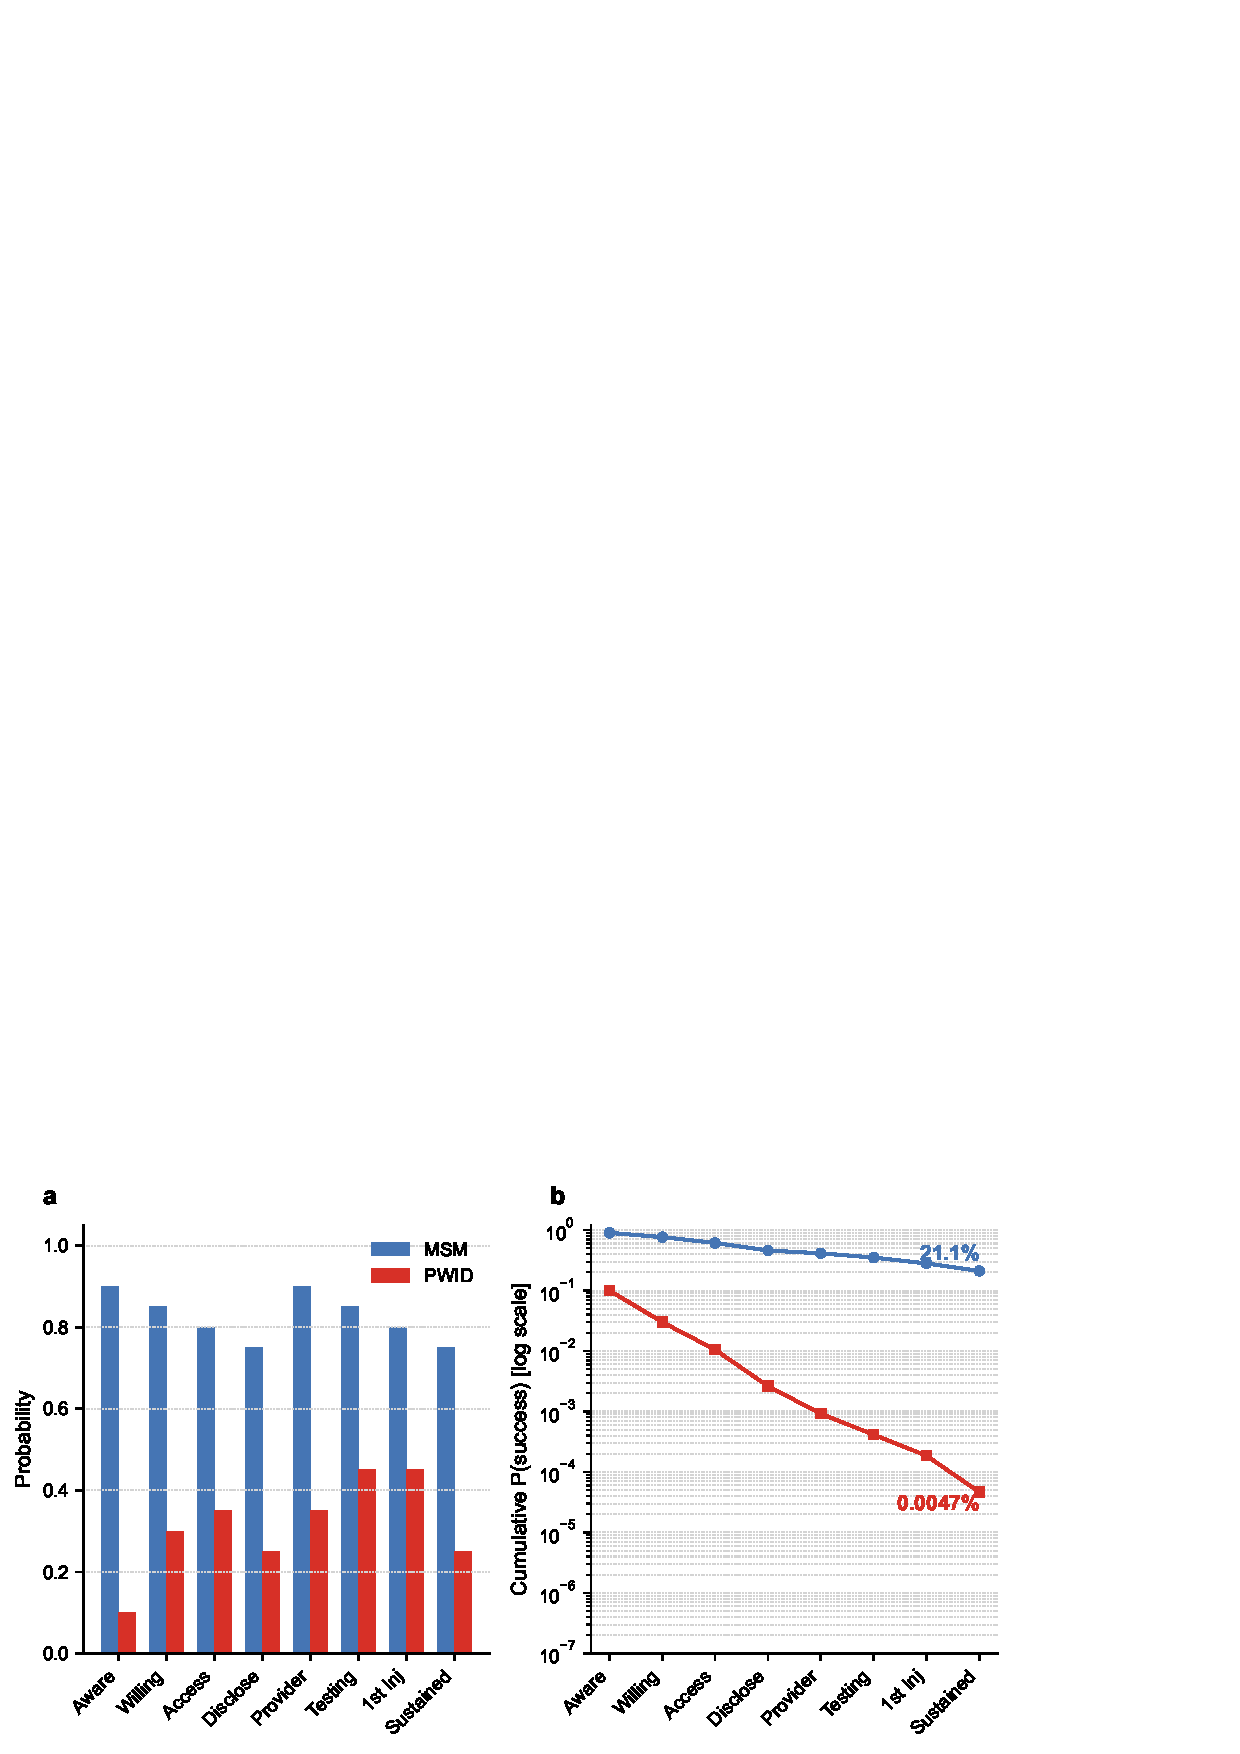
\includegraphics[width=\textwidth]{Fig1_CascadeComparison.png}
\caption{\textbf{Figure 1. LAI-PrEP Cascade Comparison: MSM vs PWID.}}
\label{fig:cascade}
\end{figure}

\begin{figure}[ht]
\centering
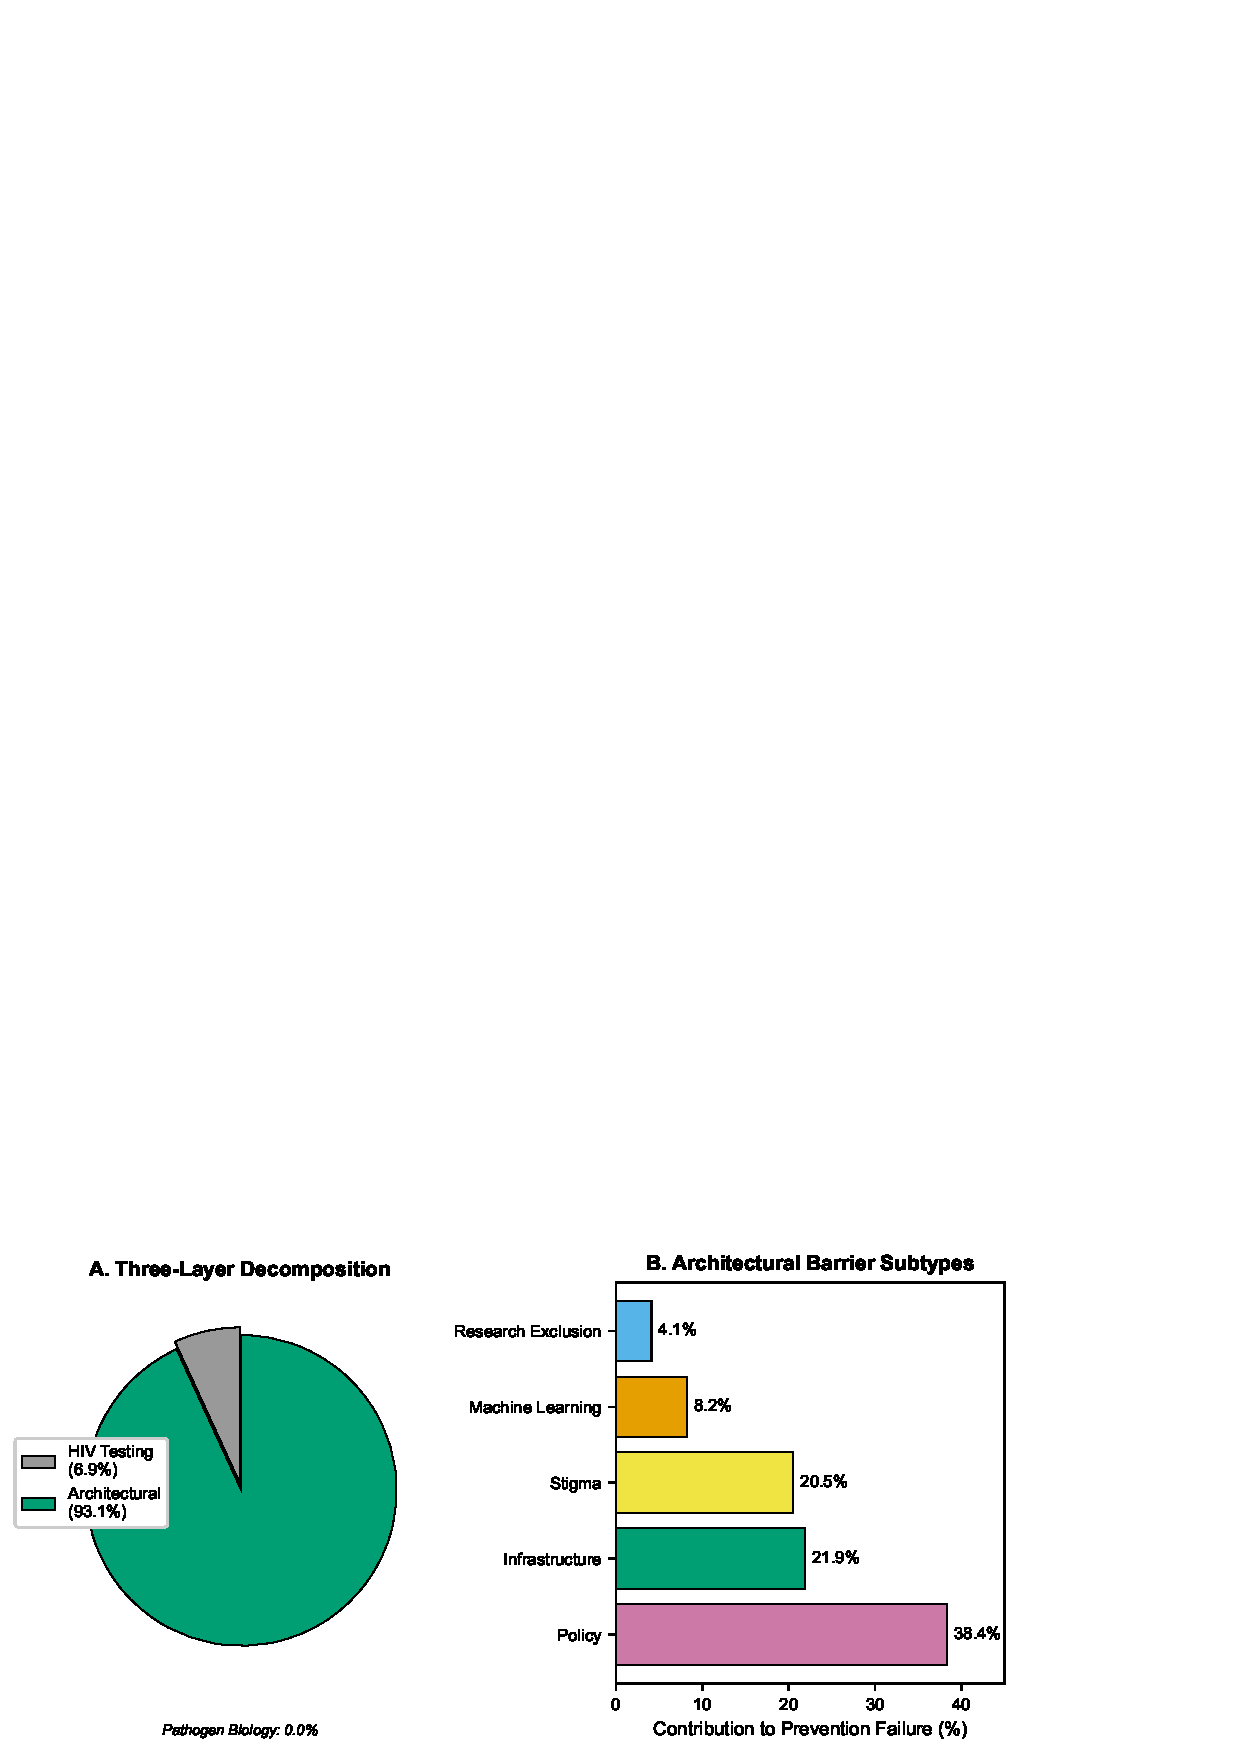
\includegraphics[width=\textwidth]{Fig2_BarrierDecomposition.png}
\caption{\textbf{Figure 2. Three-Layer Barrier Decomposition.}}
\label{fig:barriers}
\end{figure}

\begin{figure}[ht]
\centering
\includegraphics[width=\textwidth]{Fig3_PolicyScenarios.png}
\caption{\textbf{Figure 3. Policy Scenario Analysis.}}
\label{fig:policy}
\end{figure}

\begin{figure}[ht]
\centering
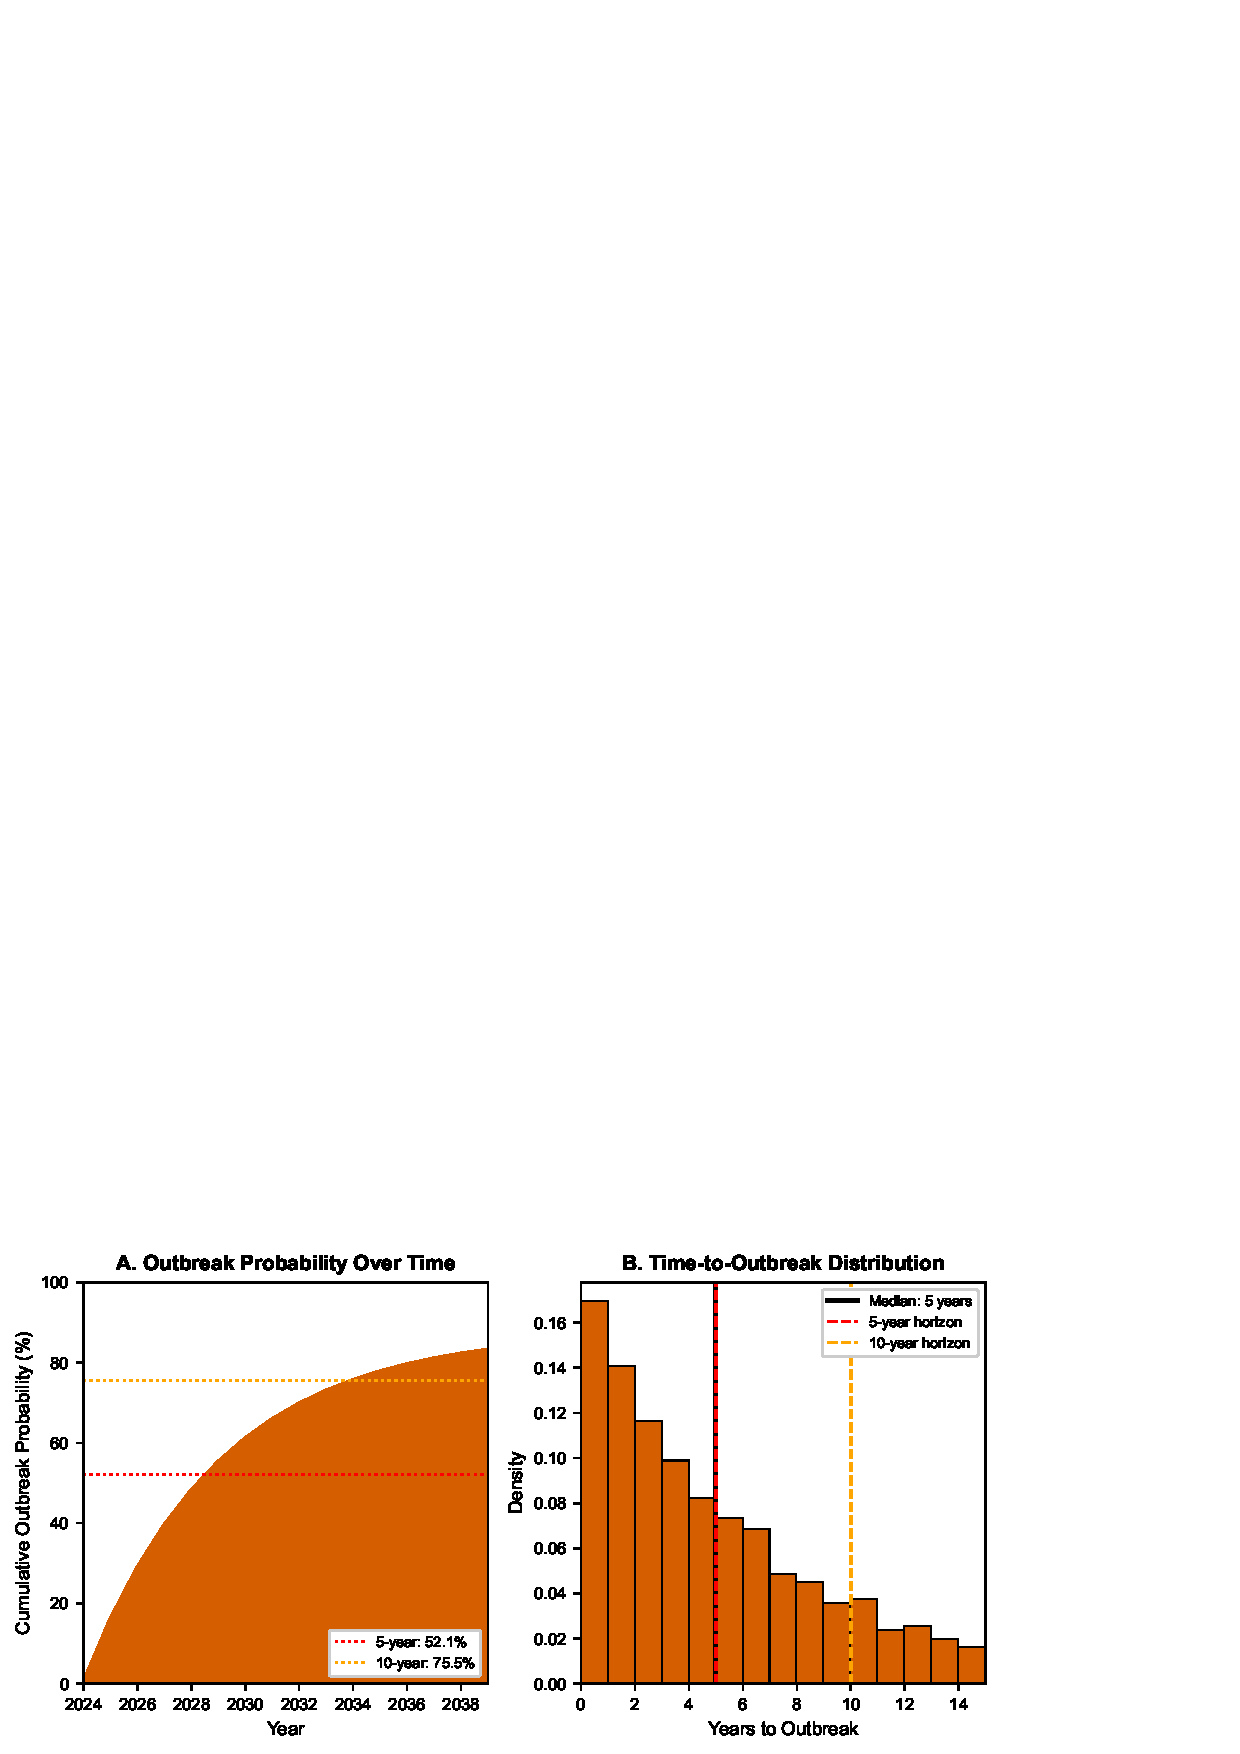
\includegraphics[width=\textwidth]{Fig4_StochasticAvoidance.png}
\caption{\textbf{Figure 4. Stochastic Avoidance Failure Prediction.}}
\label{fig:stochastic}
\end{figure}

\begin{figure}[ht]
\centering
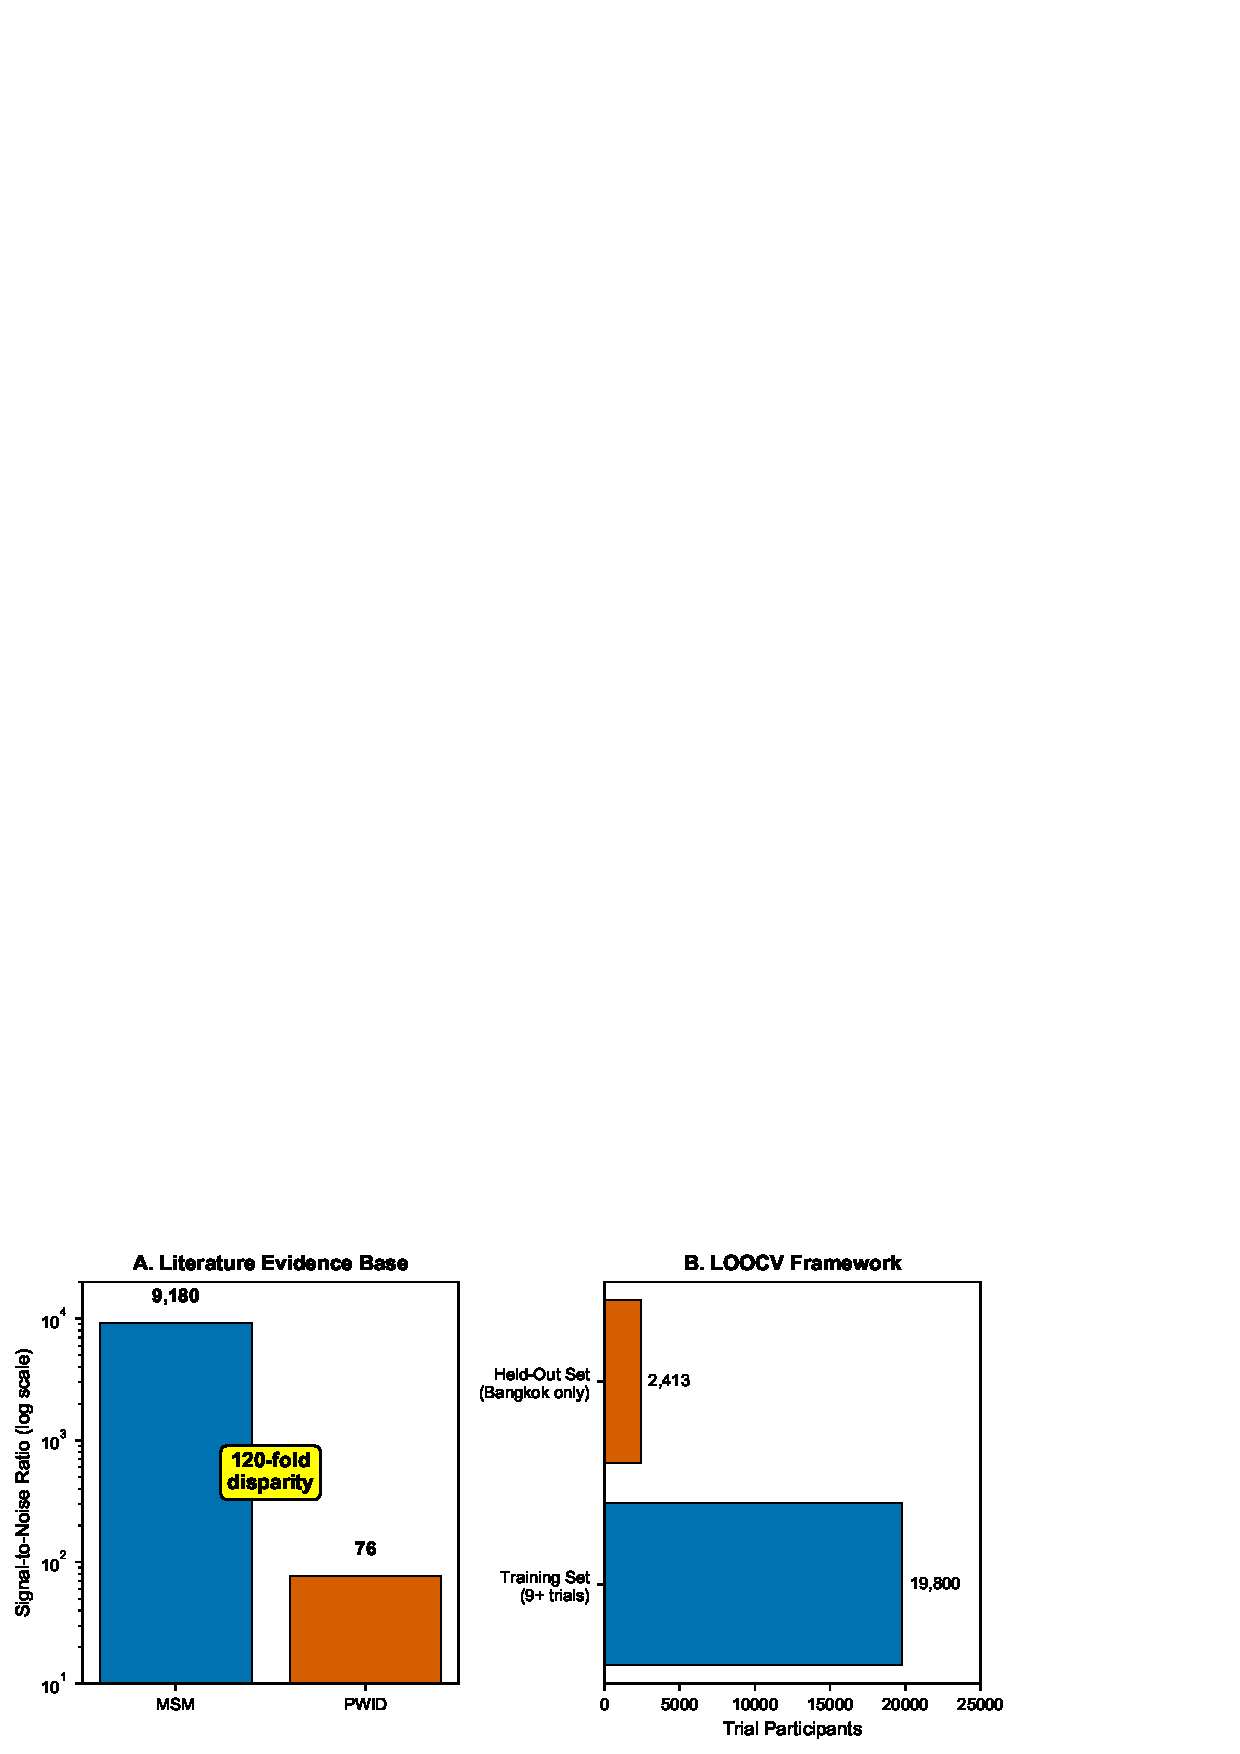
\includegraphics[width=\textwidth]{Fig5_SNR_LOOCV.png}
\caption{\textbf{Figure 5. Signal-to-Noise Ratio Disparity.}}
\label{fig:snr}
\end{figure}

\begin{figure}[ht]
\centering
\includegraphics[width=0.9\textwidth]{Fig1_FeedbackLoop.png}
\caption{\textbf{Figure 6. Algorithmic Negative Feedback Loop.}}
\label{fig:feedback}
\end{figure}

\newpage

% FIGURE LEGENDS
\section*{Figure Legends}

\textbf{Figure 1. LAI-PrEP Cascade Comparison: MSM vs PWID.} Step-wise cascade probabilities for MSM (75--95\% per step, 21.1\% completion) versus PWID (10--45\% per step, 0.0047\% completion) receiving identical pharmacological intervention. Under current policy, 90\% of PWID fail at awareness.

\textbf{Figure 2. Three-Layer Barrier Decomposition.} Attribution of prevention failure: pathogen biology 0.0\%, HIV testing 6.8\%, architectural failures 93.2\%. Within architectural failures: policy 38.4\%, infrastructure 21.9\%, stigma 20.5\%, machine learning 8.2\%, research exclusion 4.1\%. Pathogen biology contributes 0.0\% because cascade attrition prevents individuals from reaching points where biological constraints apply.

\textbf{Figure 3. Policy Scenario Analysis.} P(\Rzero{}=0) across eight scenarios from Current Policy (0.00\%) to Theoretical Maximum (19.92\%), with MSM comparison (16.30\%). No single intervention achieves meaningful improvement; multiplicative cascade requires comprehensive intervention.

\textbf{Figure 4. Stochastic Avoidance Failure Prediction.} Cumulative outbreak probability over time: 63.3\% by 5 years, 87.6\% by 10 years. Median time to outbreak: 4.0 years nationally. Regional variation reflects differential methamphetamine penetration.

\textbf{Figure 5. Signal-to-Noise Ratio Disparity.} Quantification of machine learning training data quality. MSM: SNR = 9,180 (10,800+ participants, 9+ trials, direct evidence). PWID: SNR = 76.4 (2,413 participants, 1 trial, extrapolated evidence). Disparity: 120-fold. For LAI-PrEP specifically, PWID SNR is undefined (zero participants). See Supplement S1 for derivation.

\textbf{Figure 6. Algorithmic Negative Feedback Loop.} Mechanism by which training data exclusion produces systematic algorithmic deprioritization. Trial exclusion $\rightarrow$ inadequate training data $\rightarrow$ algorithmic deprioritization $\rightarrow$ reduced access $\rightarrow$ poor outcomes $\rightarrow$ reinforced exclusion. This self-perpetuating cycle cannot be interrupted at downstream nodes; intervention requires addressing root cause (trial inclusion).

\newpage

% SUPPLEMENTARY FIGURES
\section*{Supplementary Figures}

\begin{figure}[ht]
\centering
\includegraphics[width=\textwidth]{FigS1_MethTrajectories.png}
\caption{\textbf{Supplementary Figure 1. Regional Methamphetamine Prevalence Trajectories.} Projected prevalence 2018--2040 across U.S. regions. Pacific Northwest: 35\% baseline. Appalachia: 25\% baseline, 4\%/year growth. Northeast Urban: 12\% baseline, 5\%/year growth (fastest).}
\label{fig:s1}
\end{figure}

\begin{figure}[ht]
\centering
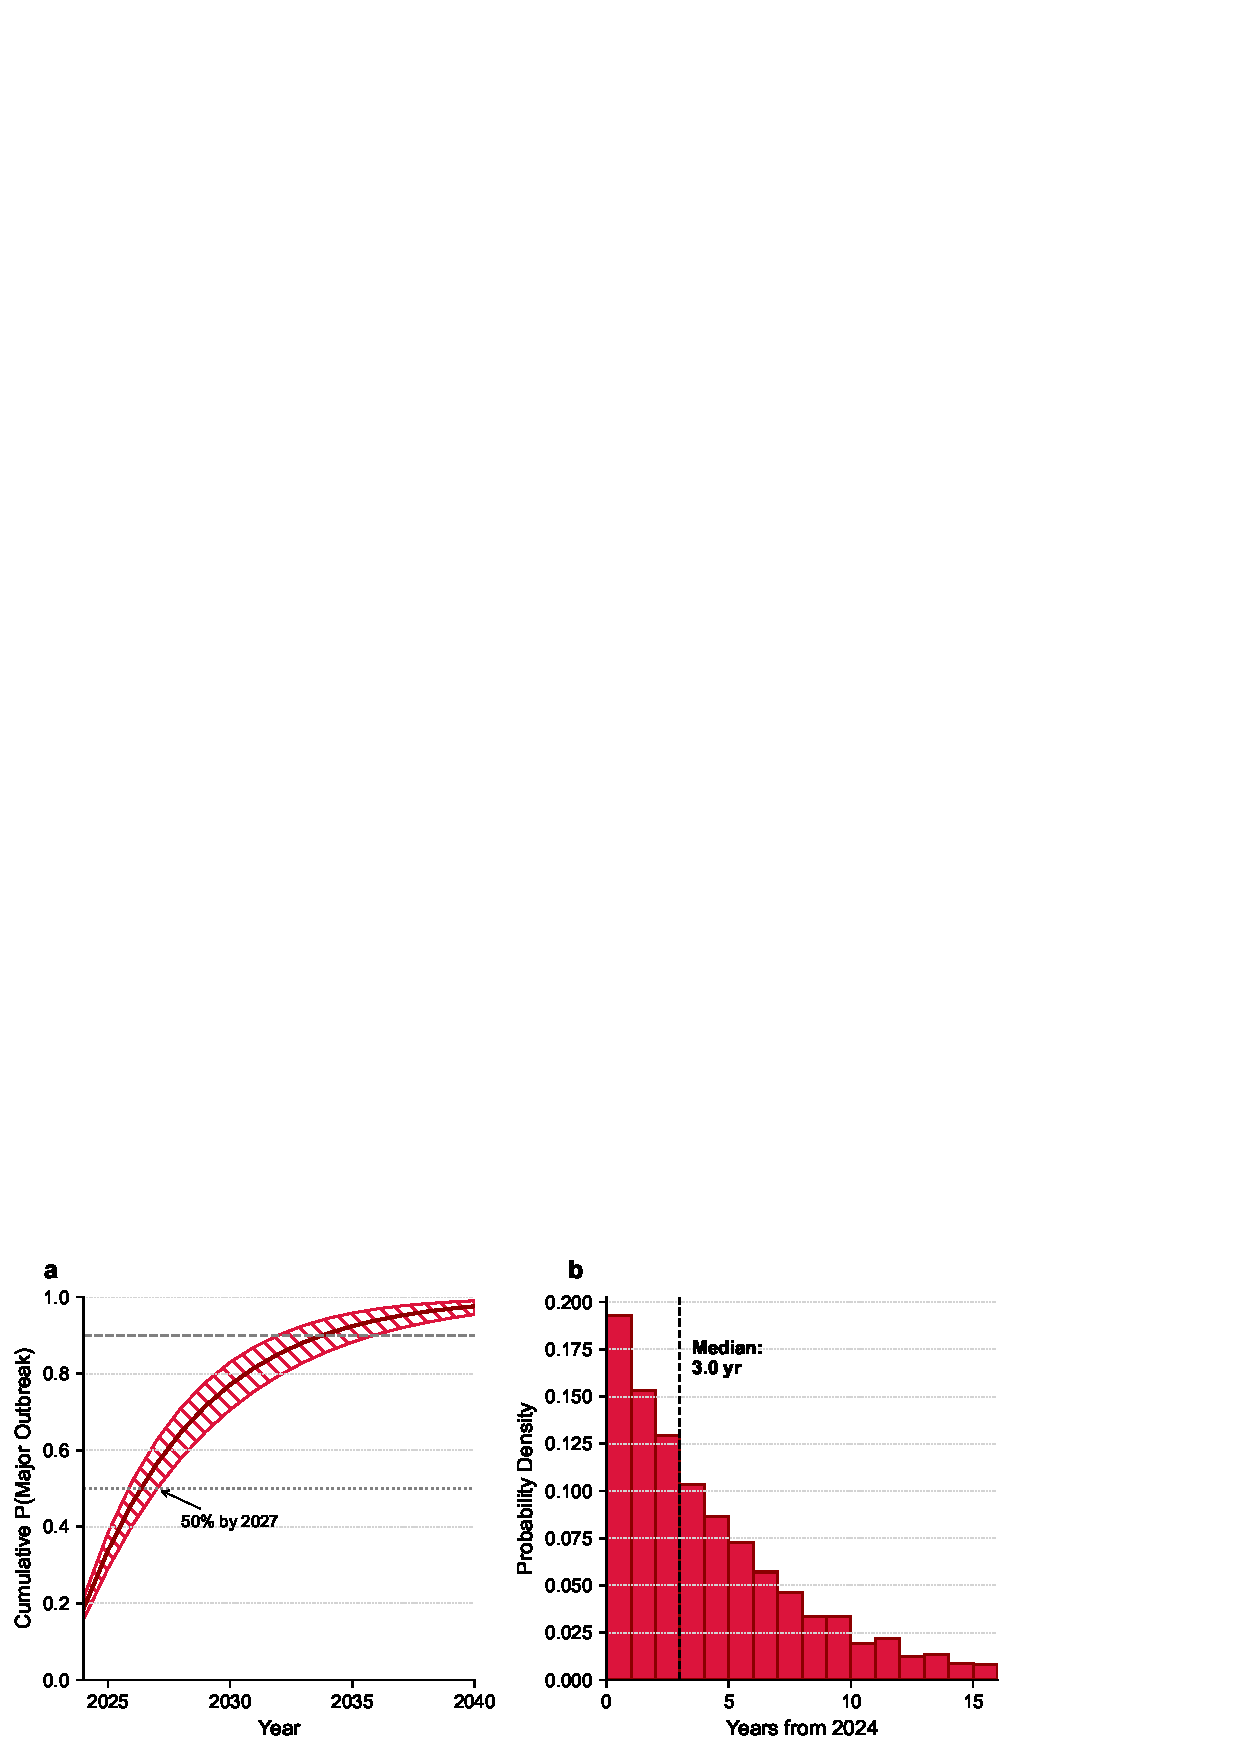
\includegraphics[width=\textwidth]{FigS2_OutbreakForecast.png}
\caption{\textbf{Supplementary Figure 2. Outbreak Probability Forecast.} Cumulative probability with 90\% confidence interval from Monte Carlo simulation (n=10,000). 50\% threshold crossed at year 4; 90\% threshold crossed at year 12.}
\label{fig:s2}
\end{figure}

\begin{figure}[ht]
\centering
\includegraphics[width=\textwidth]{FigS3_TornadoDiagram.png}
\caption{\textbf{Supplementary Figure 3. Tornado Diagram: Parameter Sensitivity.} Top parameters ranked by impact on 5-year outbreak probability. Most influential: baseline outbreak probability ($\pm$49.8pp), critical network threshold ($\pm$17.8pp), methamphetamine network multiplier ($\pm$16.6pp).}
\label{fig:s3}
\end{figure}

\begin{figure}[ht]
\centering
\includegraphics[width=\textwidth]{FigS4_ScenarioComparison.png}
\caption{\textbf{Supplementary Figure 4. Policy Scenario Outbreak Comparison.} 5-year outbreak probability and median time to outbreak by intervention scenario. Current policy: 57\%, 4.5 years. Full harm reduction: 41\%, 7.0 years.}
\label{fig:s4}
\end{figure}

\begin{figure}[ht]
\centering
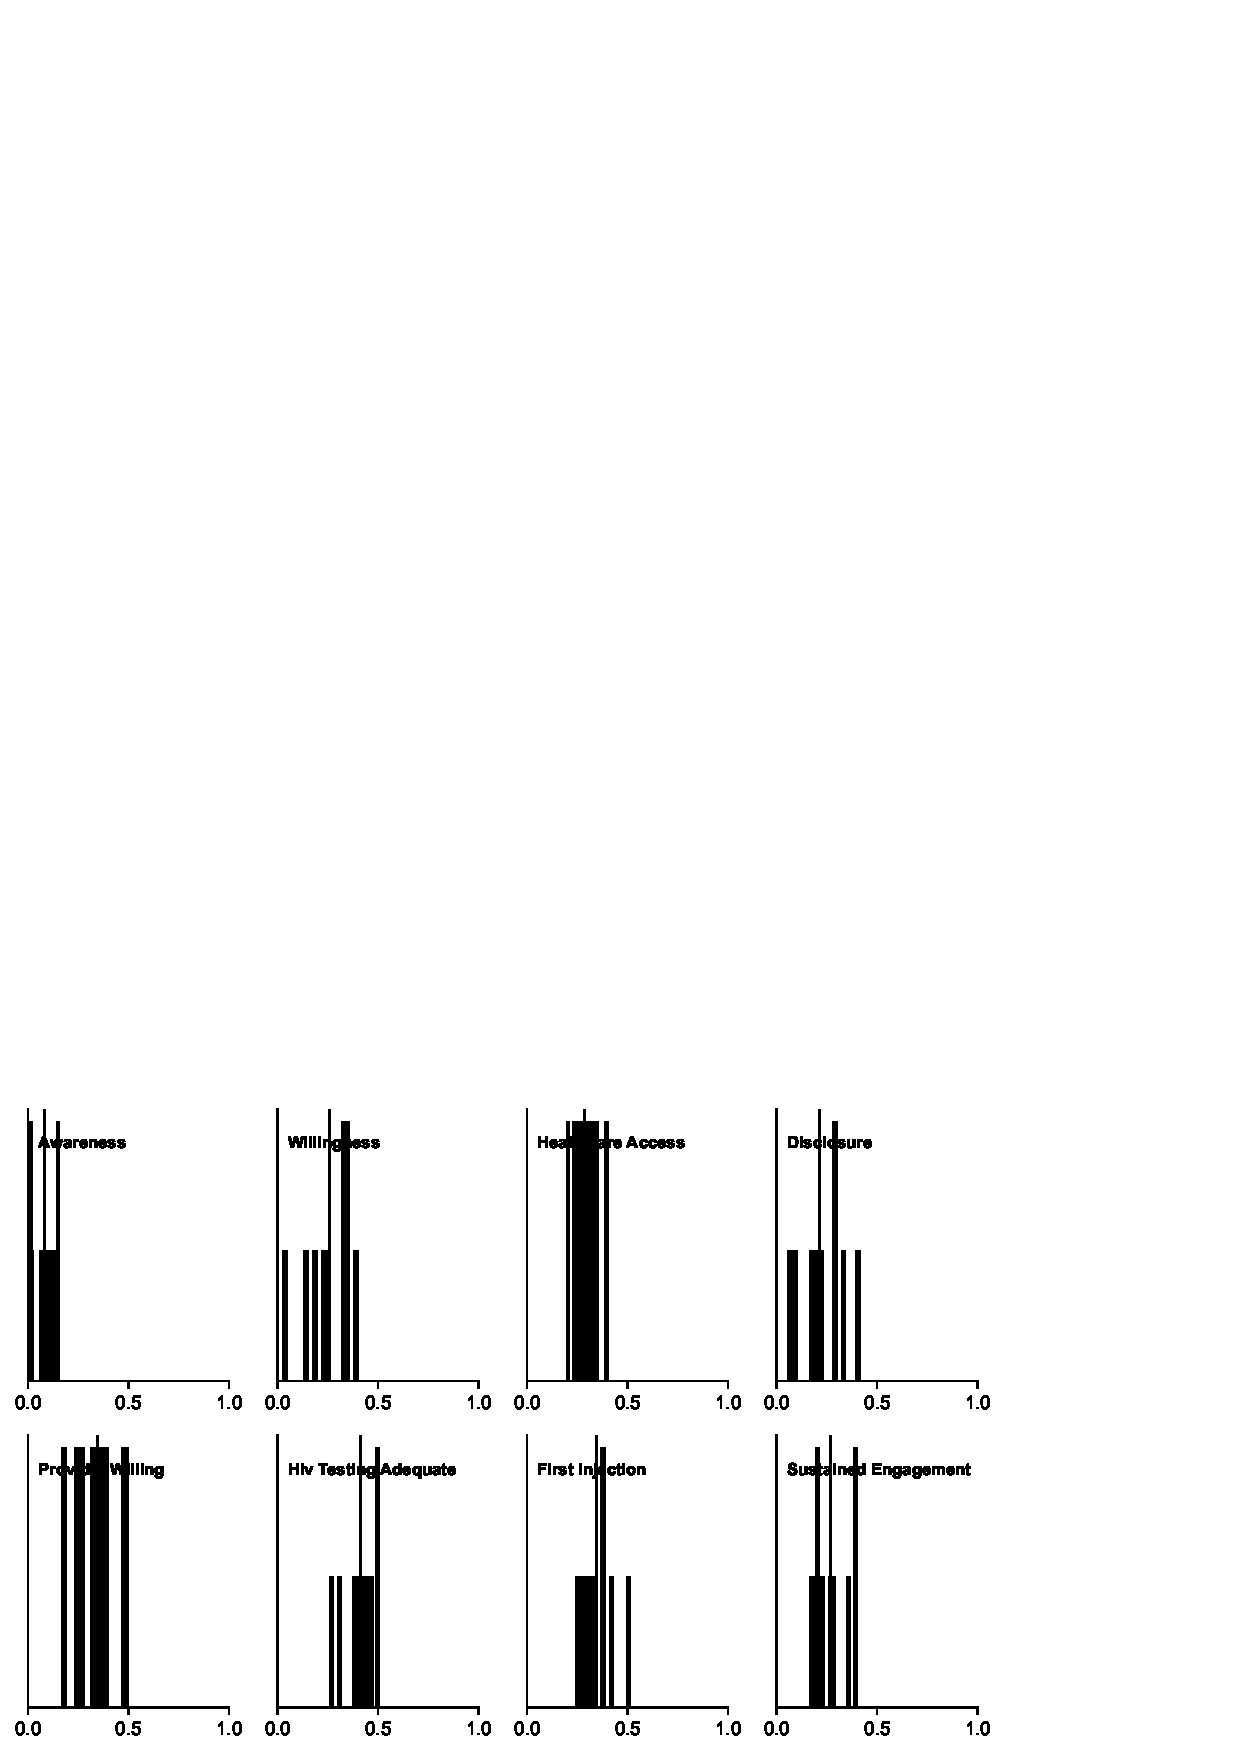
\includegraphics[width=\textwidth]{FigS5_CascadeUncertainty.png}
\caption{\textbf{Supplementary Figure 5. Cascade Step Probability Distributions.} Distributions from probabilistic sensitivity analysis (n=1,000 samples). Mean, 5th, and 95th percentiles marked.}
\label{fig:s5}
\end{figure}

\begin{figure}[ht]
\centering
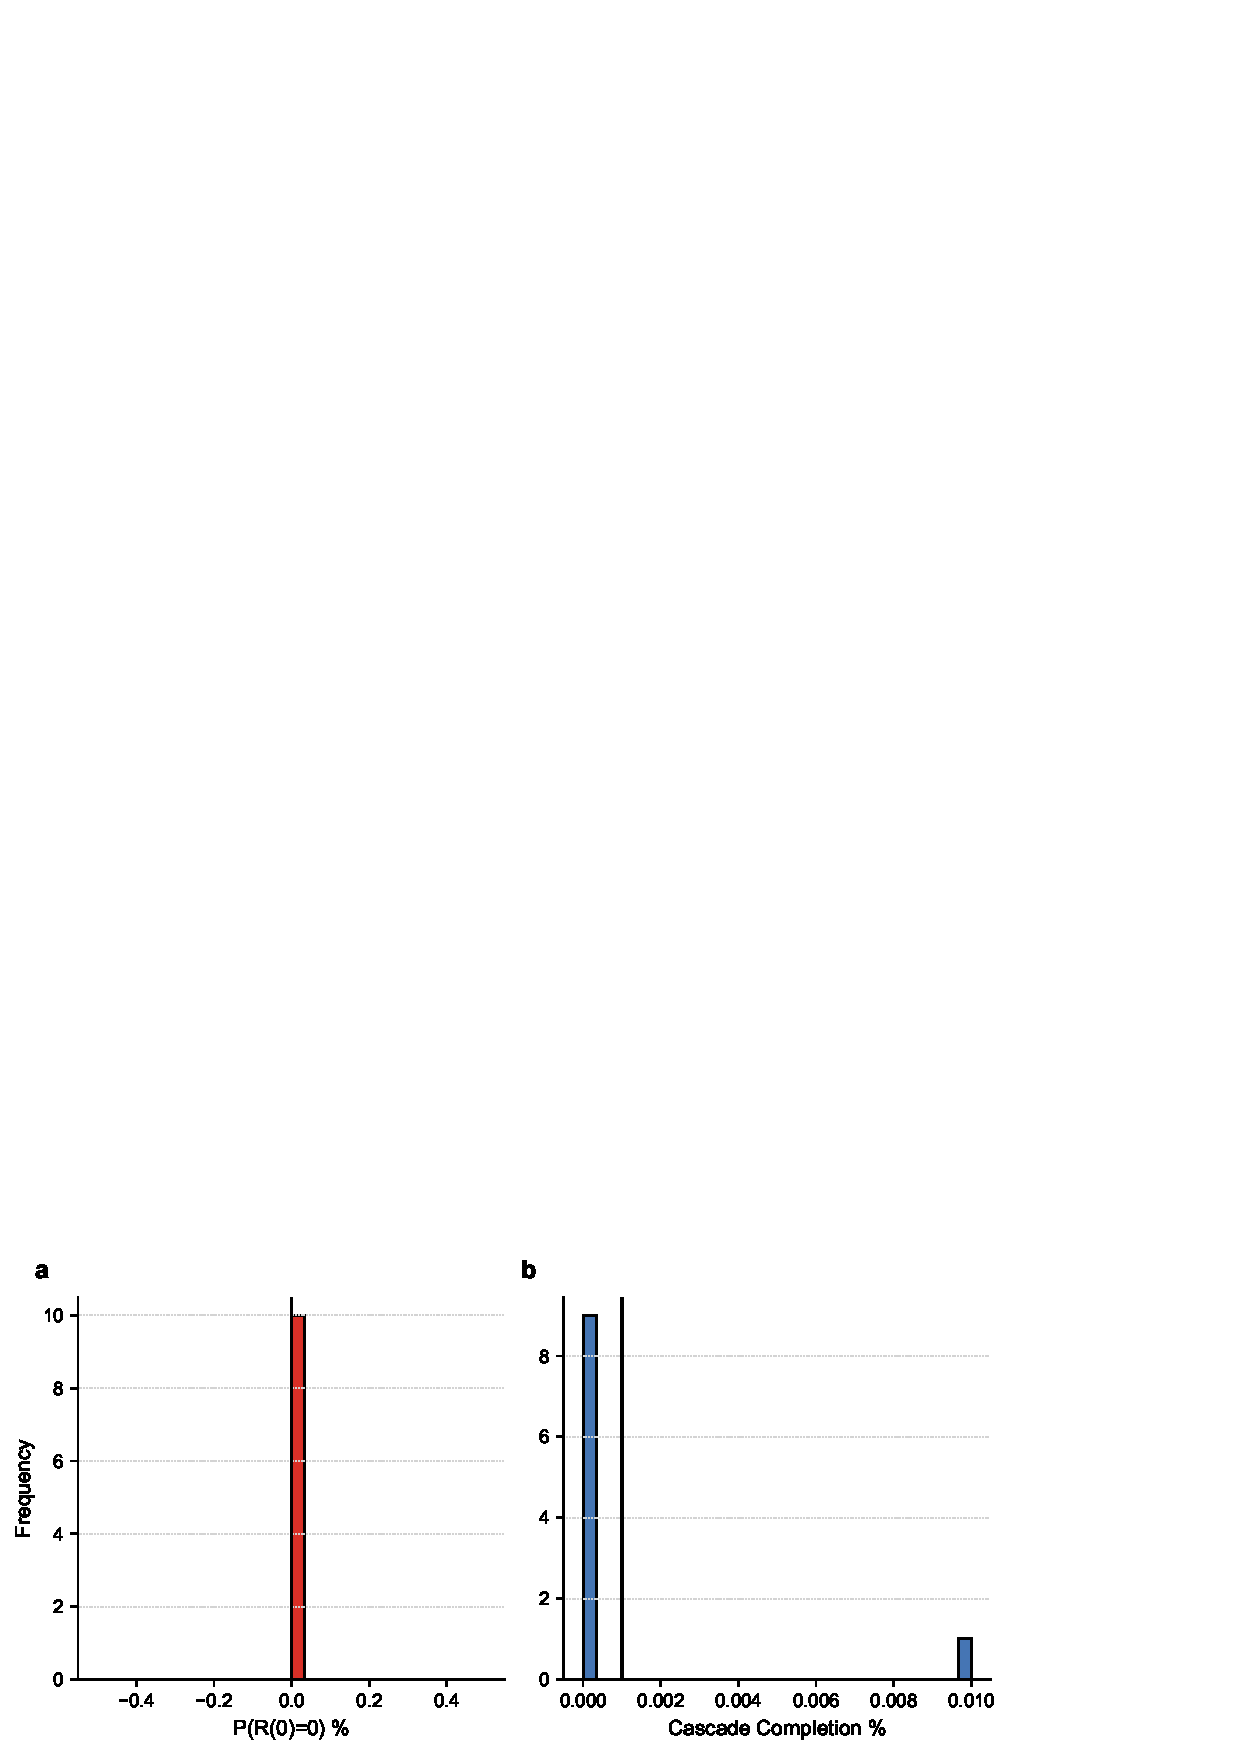
\includegraphics[width=\textwidth]{FigS6_R0ZeroDistribution.png}
\caption{\textbf{Supplementary Figure 6. P(\Rzero{}=0) Distribution from PSA.} Robustness demonstration: mean 0.0005\%, 90\% CI (0.00\%, 0.00\%) across 1,000 parameter samples.}
\label{fig:s6}
\end{figure}

\begin{figure}[ht]
\centering
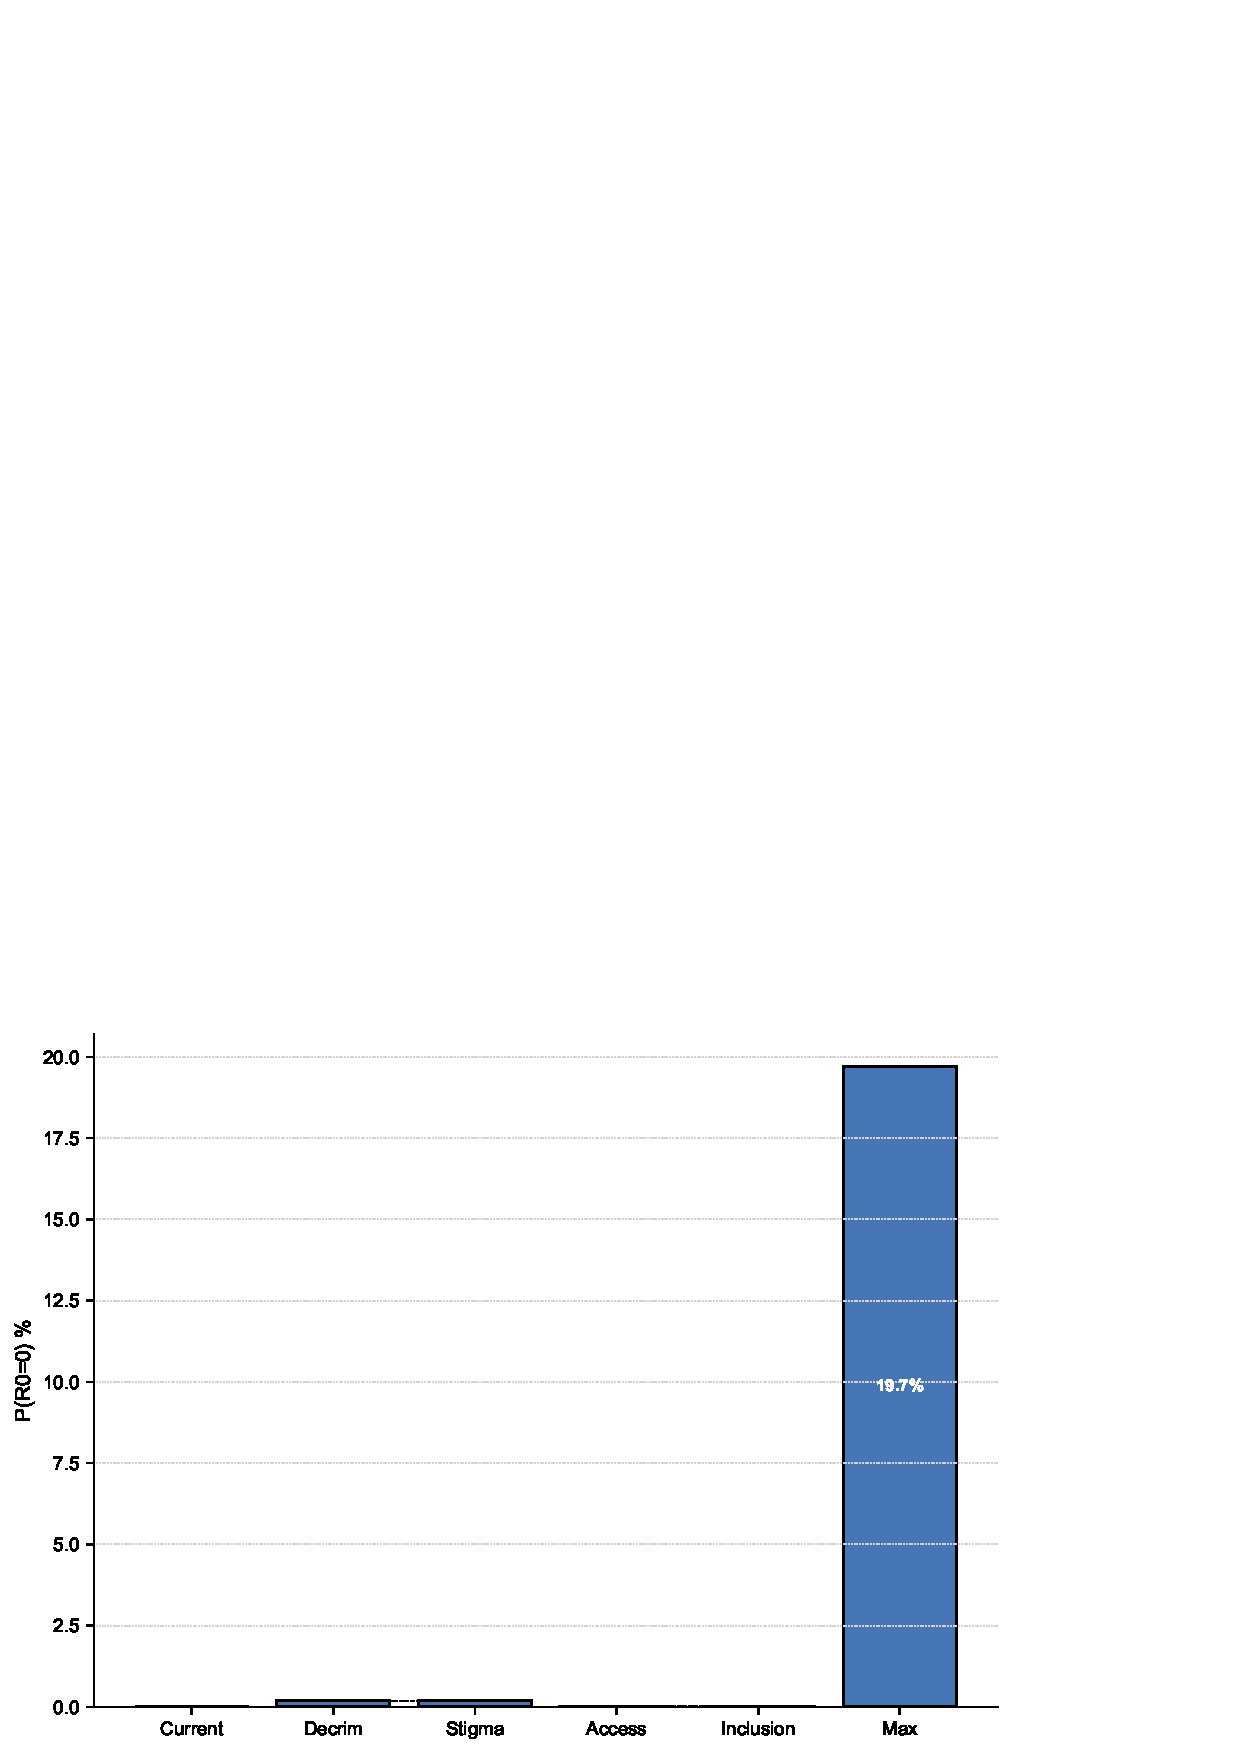
\includegraphics[width=\textwidth]{FigS7_BarrierRemoval.png}
\caption{\textbf{Supplementary Figure 7. Barrier Removal Waterfall Analysis.} Incremental effects of removing specific barrier types on P(\Rzero{}=0). No criminalization: +0.23pp. No stigma: +0.01pp. Low-barrier access: +0.02pp. Full research inclusion: +0.004pp. All barriers removed: 19.88\%.}
\label{fig:s7}
\end{figure}

\begin{figure}[ht]
\centering
\includegraphics[width=0.8\textwidth]{FigS8_StepImportance.png}
\caption{\textbf{Supplementary Figure 8. Cascade Step Importance.} Improvement in P(\Rzero{}=0) if each step fixed to 99\%. No single step achieves epidemic control; multiplicative cascade requires simultaneous intervention.}
\label{fig:s8}
\end{figure}

\newpage

% REFERENCES
\bibliographystyle{unsrtnat}
\bibliography{unified_MD}

\end{document}
